\documentclass{article}

\usepackage{tikz}
\usetikzlibrary{automata,positioning}
\begin{document}
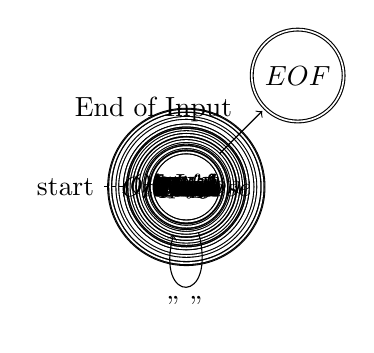
\begin{tikzpicture}[shorten >=1pt,node distance=2cm,on grid,auto]
   \node[state,initial] (s0)   {$Start$}; 
   \node[state, accepting] (eof) [above right = of s0] {$EOF$};
   \node[state, accepting] (func)   {$Func$};
   \node[state, accepting] (identifier)   {$Identifier$};
   \node[state, accepting] (main)   {$Main$};
   \node[state, accepting] (l_paren)   {$L_Paren$};
   \node[state, accepting] (r_paren)   {$R_Paren$};
   \node[state, accepting] (l_curly)   {$L_Curly$};
   \node[state, accepting] (r_curly)   {$R_Curly$};
   \node[state, accepting] (comma)   {$Comma$};
   \node[state, accepting] (colon)   {$Colon$};
   \node[state, accepting] (return)   {$Return$};
   \node[state, accepting] (semicolon)   {$Semicolon$};
   \node[state, accepting] (int)   {$Int$};
   \node[state, accepting] (bool)   {$Bool$};
   \node[state, accepting] (if)   {$If$};
   \node[state, accepting] (else)   {$Else$};
   \node[state, accepting] (while)   {$While$};
   \node[state, accepting] (assign)   {$Assign$};
   \node[state, accepting] (print)   {$Print$};
   \node[state, accepting] (equals)   {$Equals$};
   \node[state, accepting] (greater)   {$Greater$};
   \node[state, accepting] (plus)   {$Plus$};
   \node[state, accepting] (minus)   {$Minus$};
   \node[state, accepting] (mult)   {$Mult$};
   \node[state, accepting] (int_lit)   {$Int_Lit$};
   \node[state, accepting] (true)   {$True$};
   \node[state, accepting] (false)   {$False$};
   \node[state, accepting] (not)   {$Not$};
   \node[state, accepting] (and)   {$And$};
   \node[state, accepting] (or)   {$Or$};
   \node[state, accepting] (question)   {$Question$};
   \node[state, accepting] (then)   {$Then$};
   \node[state, accepting] (otherwise)   {$Otherwise$};
   \path[->] 
    (s0) edge  [loop below] node {" "} (s0)
        edge  node  {End of Input} (eof);
\end{tikzpicture}
\end{document}  
